We varied the number of demand and supply sites to see how the 
different methods scaled across these. The number of years considered was kept constant at 22, 
the full length of data available. Subsets of data obtained were checked for feasibility before 
attempting to solve. The results of trial runs of 
different sizes are show in table \ref{tab:uk_performance}.


\begin{table}[h]
    \centering
    \caption{Performance Comparison of LR Heuristic and to ESLP}
    \label{tab:uk_performance}
    \renewcommand{\arraystretch}{1.2}
    \setlength{\tabcolsep}{10pt} % Adjust column spacing
    
    \begin{tabular}{cc ccc c}
        \toprule
        \textbf{NS} & \textbf{ND} & \multicolumn{3}{c}{\textbf{LR Heuristic}} & \multicolumn{1}{c}{\textbf{ESLP}} \\
        \cmidrule(lr){3-5} \cmidrule(lr){6-6}
         & & \textbf{Time (s)} & \textbf{Gap} & \textbf{Iterations}& \textbf{Time (s)} \\
        \midrule
        3 & 3 & 0.13 & 0 & 1 & 0.13 \\
        10 & 10 & 0.32 & 0.02 & 5 & 0.16\\
        10 & 20 & 5.81 & 0.01 & 8 & 0.22 \\
        10 & 50 & 0.3 & 0.01 & 8 & 0.24\\
        20 & 10 & 9.98  & 0.01 & 23 & 0.18\\
        30 & 10 & 13.77  & 0.02 & 23 & 0.23\\
        50 & 20 & 67.64 & 0.01 & 42 & 0.54 \\
        50 & 50 & 100.16 & 0.02 & 50 & 1.05 \\
        100 & 100 & 600.07& 0.01 & 50 & 4.57 \\
        200 & 200 & 1800.02 & 0.02 & 80 & 20.2 \\

        \bottomrule
    \end{tabular}

    \vspace{5pt}
    \footnotesize NS = Number of Supply Sites, ND = Number of Demand Sites. 
    Gap = (UB - LB)/UB.
\end{table}




The LR Heurisic clearly takes significantly
longer to reach a solution than simply solving
the ESLP directly with the Gurobi solver, scaling poorly regardless of whether
increasing supply sites or demand sites. The LR heuristic 
however did consistently converge to a tighter
bound, and given higher maximum iterations the 
gap continued to narrow in all cases.

We also present some of the figures illustrating the 
power lines the ESLP solutions converged on \ref{fig:uk_cases}. Figures with more sites were
too connected for differing sites to be discernable. 

Some comments on what this model suggested for UK renewable energy infrastructure.
The model favoured Hydro Power stations over any other. This is likely due to 
transmission being relatively cheap, exacerbated by the use of shortest distances 
to arrive at transmission costs, and power generation being cheapest for hydro power stations
alongside large amounts of capacity, even despite their higher setup cost.

\begin{figure}[H]
    \centering
    \begin{subfigure}[b]{0.45\textwidth}
        \centering
        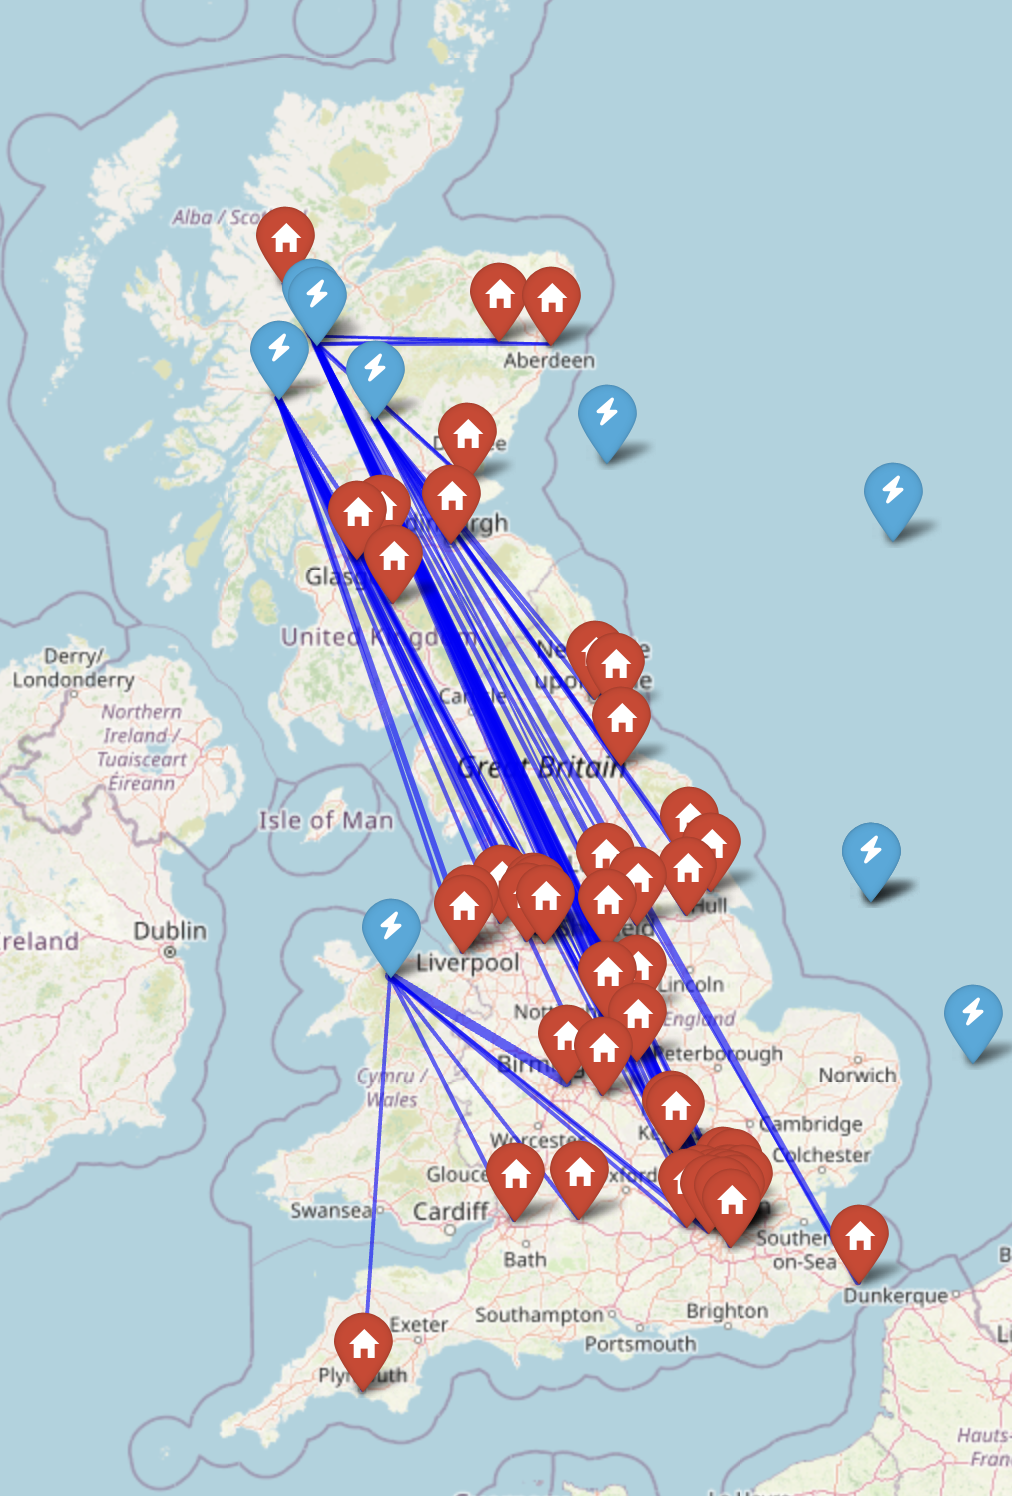
\includegraphics[width=\textwidth]{figures/test_8_base.png}
        \caption{Case with 50 demand sites and 10 supply sites}
        \label{fig:uk_case_1}
    \end{subfigure}
    \hfill
    \begin{subfigure}[b]{0.45\textwidth}
        \centering  
        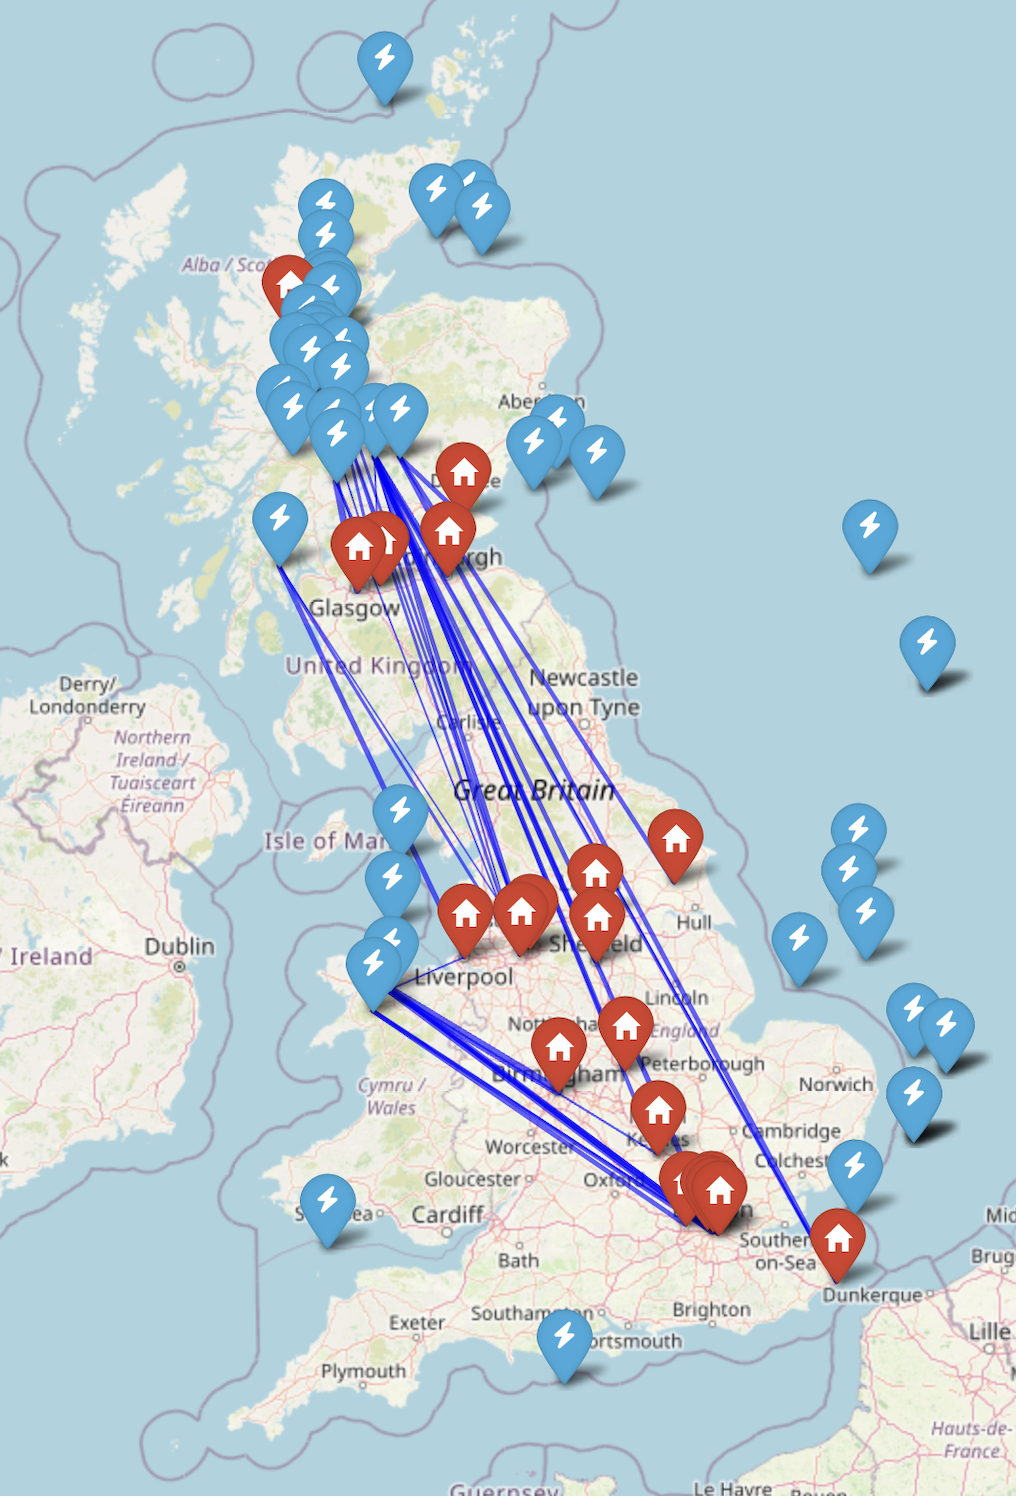
\includegraphics[width=\textwidth]{figures/test_12_base.png}
        \caption{Case with 20 demand sites and 50 supply sites}
        \label{fig:uk_case_2}
    \end{subfigure}
    \caption{UK Energy Networks found as solutions to the ESLP}
    \label{fig:uk_cases}
\end{figure}

